\documentclass[mathserif, aspectratio=169]{beamer}

\usepackage{movie15}
\usepackage{psfrag,graphicx}
\usepackage{amsmath}
\usepackage[absolute,overlay]{textpos}

\graphicspath{{figs/}}

\usetheme{Boadilla}
\makeatother
\setbeamertemplate{footline}[frame number]

\usepackage{graphicx}
\usepackage{caption}
\usepackage{subcaption}
\captionsetup{compatibility=false}
\usepackage{amsmath} 
\usepackage{amssymb} 
\usepackage{amsthm}  
\usepackage{bm}
\usepackage{lipsum}
\usepackage[linesnumbered, ruled]{algorithm2e}
\usepackage{color}
\newtheorem{assumption}{Assumptions}
\newtheorem{prop}{Proposition}
\newtheorem{defn}{Definition}
\newtheorem{thm}{Theorem}
\newtheorem{lem}{Lemma}
\newtheorem{cor}{Corollary}
\newtheorem{sol}{Decentralized Solution}
\newtheorem{thresh}{$\epsilon$-thresholding}
\definecolor{light-gray}{gray}{0.8}
\usepackage{textcomp}

\newcommand{\backupbegin}{
   \newcounter{finalframe}
   \setcounter{finalframe}{\value{framenumber}}
}
\newcommand{\backupend}{
   \setcounter{framenumber}{\value{finalframe}}
}
\newcommand{\norm}[1]{\left\lVert #1 \right\rVert}

\makeatletter
\setbeamertemplate{navigation symbols}{}



\title[Lecture 19] % (optional, use only with long paper titles)
{Data, Environment and Society: \\{Lecture 19: Classification and regression trees}}


%\subtitle
%{Include Only If Paper Has a Subtitle}

\author[ER131: Data, Environment and Society] 
{Instructor: Duncan Callaway\\
GSI: Salma Elmallah} 

\vspace{-20mm}
\institute[UC Berkeley] % (optional, but mostly needed)
 {\small{ \bf November 5, 2019}}


\date[November 5, 2019]

\begin{document}

\frame{  
 \begin{columns}
 \column{0.6\textwidth}
   \titlepage
 \column{0.4\textwidth}
\vspace{-0mm}
\begin{figure}
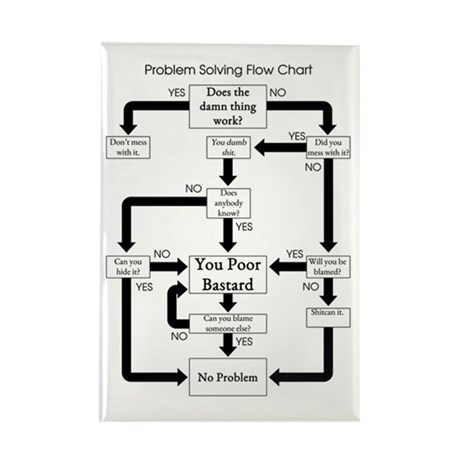
\includegraphics[width=\textwidth]{decision_tree}
\caption*{\tiny https://thenexttobestblogever.wordpress.com/2009/11/07/problem-solving-flowchart-2/}
\end{figure}
 \end{columns}
}


\begin{frame}{Today's objectives}


\begin{itemize}
\item Wrap up regression trees
\begin{itemize}
\item How to choose with cross validation
\end{itemize}
\item Classification trees
\begin{itemize}
\item Same as regression, just different loss functions
\end{itemize}
\item Boosting, bagging and random forests
\end{itemize}

\textbf{Reading}
\begin{itemize}
\item Today: ISLR Ch. 8.1 - 8.2
\item Next time: 
\begin{itemize}
	\item ISLR 9.1-9.3 (Support Vector Machines)
	\item Badger (NYT article on algorithm discrimination)
\end{itemize}
\end{itemize}

\textbf{Announcements}
\begin{itemize}
\item Guest lecture -- Elinor Benami, author of one of the first papers we read this semester.
\item Exam review 11/14 in class, 11/18 in lab.
\item Exam 11/19
\end{itemize}

\end{frame}



\begin{frame}{Last time: where should the splits be?}

Then we partition any region by choosing $j$ and $s$ as follows:

\begin{align*}
\{j,s\} = \arg \min_{j\in J, s\in X_j} \sum_{i:x_i\in R_1(j,s)} (y_i-\hat{y}_{R_1})^2 + \sum_{i:x_i\in R_2(j,s)} (y_i-\hat{y}_{R_2})^2
\end{align*}
where $\hat{y}_{R_k}$ is the mean of all response variables in region k.  \\~\\

It would be tedious to identify $j$ and $s$ by hand, but it's actually very quick computationally.  (Remember, there are only $n-1$ possible splits for each predictor.)
\end{frame}

\begin{frame}{Ok, we've split one predictor in two.  Now what?}

Next choose the single best split from among \textit{all} possible splits of the two new regions. \textbf{Now we'll have three regions.}\\~\\

In general, on the $n^\text{th}$ step, choose the single best possible split from among the $n$ regions, resulting in $n+1$ regions to take to the next step. \\~\\

Repeat this process until you reach a stopping criterion -- typically a maximum number of observations in each region. (For example all regions have no more than 5 observations.) \\~\\ \textbf{Call the resulting tree $T_0$.} \\~\\

\textbf{We call this approach ``greedy''} because when we do the first partition we're not thinking ahead to future partitions to evaluate it.  
\end{frame}


\begin{frame}{Example $T_0$}
\begin{columns}
\column{0.35\textwidth}
Remember, $T_0$ is the biggest tree we build.  We get there by recursively splitting until we meet a threshold (often a maximum number of observations per terminal node).
\column{0.65\textwidth}
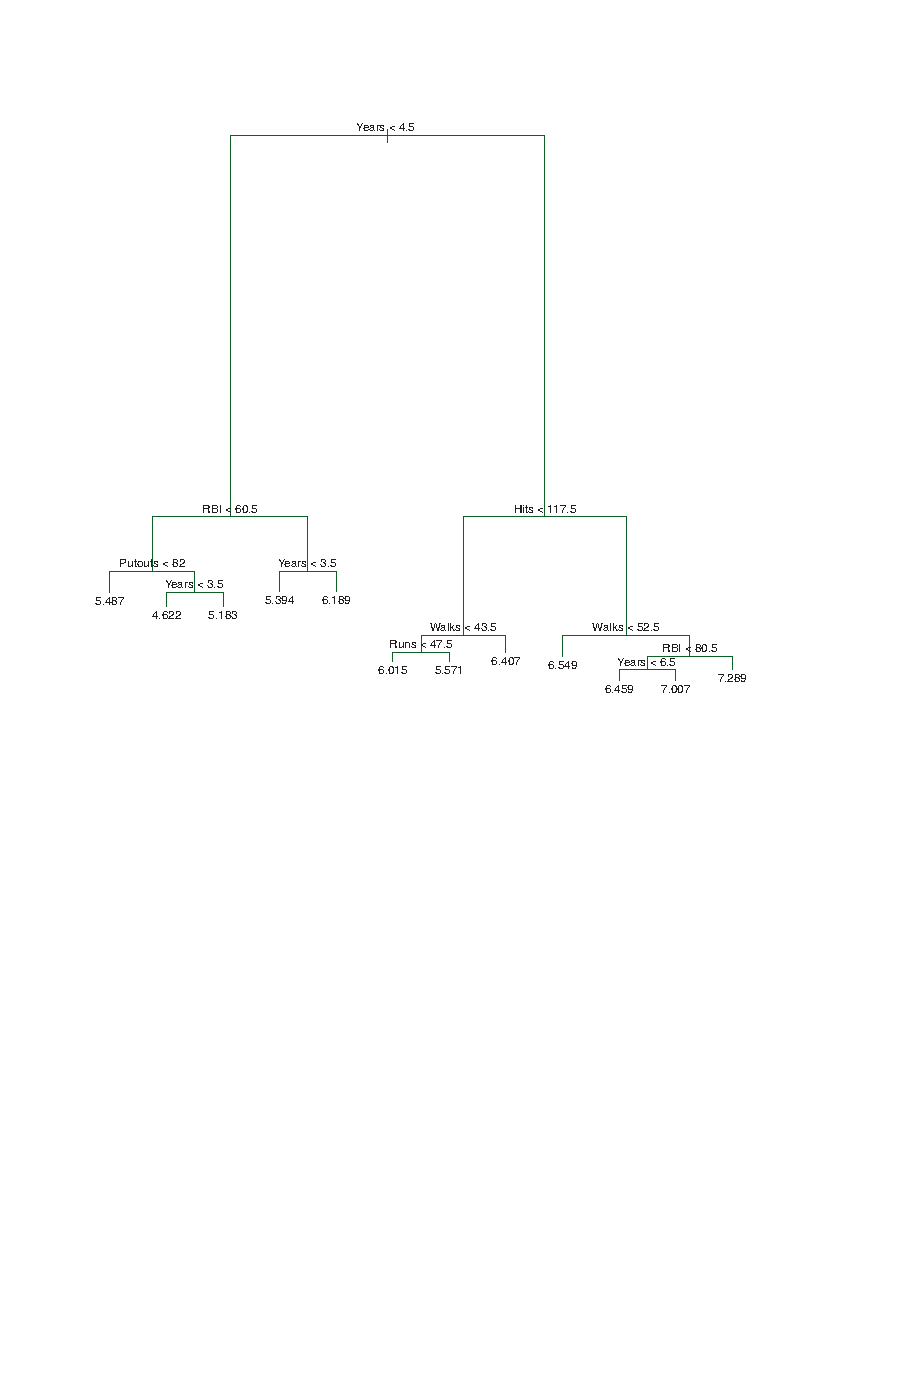
\includegraphics[height=0.9\textheight]{complex_tree}

\end{columns}

\end{frame}

\begin{frame}{Choosing the final tree, \textbf{Step 1: } ``cost complexity pruning''}

We'll test models that are \textbf{subtrees} of $T_0$. (trees that are the same as $T_0$ except they are missing some internal nodes and branches).\\~\\

We identify subtrees using \textbf{cost-complexity pruning} a.k.a. weakest link pruning:
\vspace{4mm}
\begin{itemize}
\item To get the first subtree, evaluate model performance for all subtrees with one leaf removed from $T_0$.  Choose the best one, call it $T_1$.  
\begin{itemize}
\item $R^2$ works for measuring performance
\item ...but not for categorical variables, stay tuned!
\end{itemize}
\vspace{4mm}
\item Then evaluate performance for all models with one leaf removed from $T_1$.  Choose the best, call it $T_2$.  And so on.  \\~\\
\end{itemize}

\pause

(Smart researchers have shown that this ``greedy'' approach is an optimal \textit{pruning} strategy.  But recursive binary splitting is not always optimal for growth.)

\end{frame}

\begin{frame}{Choosing the final tree, \textbf{Step 2: } Tune up your $\alpha$}
Take your set of subtrees, $T_0$ through $T_{N-2}$.  Call $|T|$ the number of terminal nodes in the tree.\\~\\

For a given $\alpha$, \textit{one} of the $T_i$ will minimize :
\begin{align*}
\sum_{m=1}^{|T|} \sum_{x_i\in R_m} (y_i-\hat{y}_{R_m})^2+\alpha|T|
\end{align*}

\begin{itemize}
\item $\alpha=0$ will choose $T_0$, the biggest tree.
\item As $\alpha$ grows you'll choose successively smaller trees.  \\~\\
\end{itemize}

\end{frame}

\begin{frame}{Quick quiz}

For a given $\alpha$, \textit{one} of the $T_i$ will minimize :
\begin{align*}
\sum_{m=1}^{|T|} \sum_{x_i\in R_m} (y_i-\hat{y}_{R_m})^2+\alpha|T|
\end{align*}

Fill in the blank:  As $\alpha$ increases, bias goes \underline{\uncover<2->{\textbf{up}}} and variance goes \underline{\uncover<2->{\textbf{down}}}.  
%
\pause
%
Bigger $\alpha$ means fewer leaves, which means more bias but less variance.   \\~\\

Though it seems unnecessary to define $\alpha$ (why not just evaluate all subtrees?), we'll see it's useful for cross validation.  
\end{frame}

\begin{frame}{The (cross validation) process}

\begin{enumerate}
\item Split your data into $K$ folds.  
\vspace{3mm}
\item Repeat this process for each fold: Withhold the fold and for remaining training data:
\begin{enumerate}
\item[\textbf{a.}] Grow a large tree via recursive binary splitting.  ``Large'' means each leaf has some pre-specified maximum number of observations (e.g. 5)
\item[\textbf{b.}] Then ``prune'' the tree via cost complexity pruning to get a sequence of subtrees.  
\item[\textbf{c.}] Choose the tree in the sequence that minimizes $\sum_{m=1}^{|T|} \sum_{x_i\in R_m} (y_i-\hat{y}_{R_m})^2+\alpha|T|$ for each of a range of values of $\alpha$.
\item[\textbf{d.}] Record the test MSE for each value of $\alpha$.
\vspace{3mm}
\end{enumerate}
\item Average the test MSE across all folds \textit{for each value of }$\alpha$, 
\vspace{3mm}
\item Choose the $\alpha$ that gives the lowest cross validated error, 
\vspace{3mm}
\item Build your final model with the chosen $\alpha$ with \textit{all the data.}
\end{enumerate}
\end{frame}

\begin{frame}{Why use $\alpha$?}

Why didn't we just evaluate cross validated error for each tree size?\\~\\

That is, is $\alpha$ just overly complicating things?\\~\\

\pause

Ans: Sometimes it might.  But it may be that across different folds we'd choose different subtrees.  $\alpha$ provides a better representation of the bias-variance tradeoff across folds.  \\~\\

But: out of convenience the book \textit{displays} results in terms of tree size rather than $\alpha$.  Argh!

\end{frame}

\begin{frame}{Results on Hitters data}
\begin{figure}
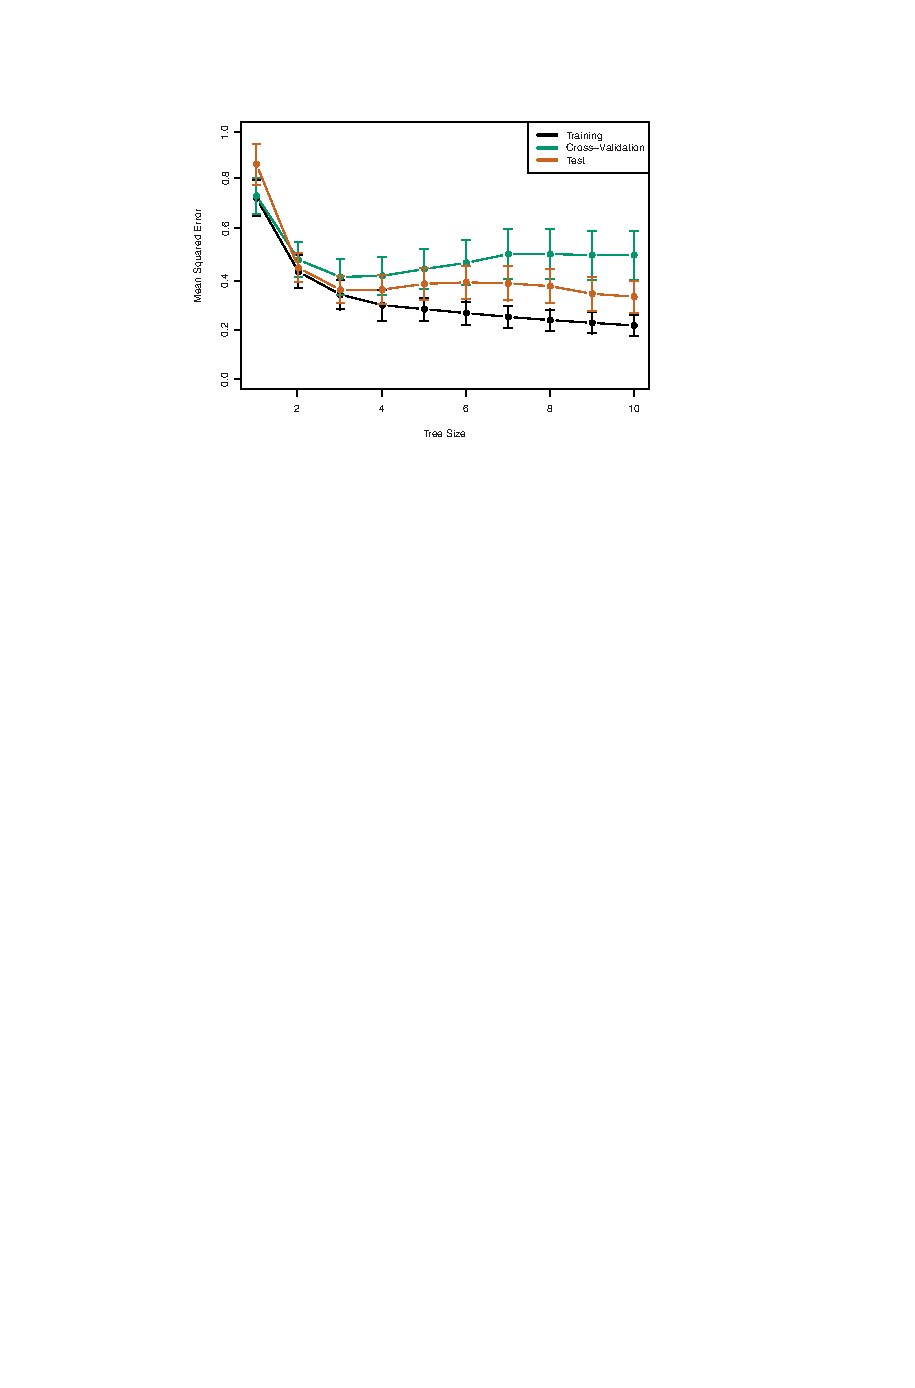
\includegraphics[width=0.8\textwidth]{MSE_vs_treesize}
\caption*{``Training'' data are 132 of the 263 original observations.  Test are the reminaining.  CV is done just on the training data -- that is the training data are split into the K folds (6 in this case).  The test data are just used for additional evaluation.}
\end{figure}
\end{frame}

\begin{frame}{Question}

Do regression trees utilize linear regression? \pause Nope.  \\~\\

What do you think their advantages are (vs LASSO or nonlinear models...)? \pause

\begin{itemize}
\item Easy to explain and non-experts can understand the results.
\item They're more like human decision-making.  Doctors like them.
\item They easily handle qualitative predictors -- no need for dummies.
\end{itemize}

\pause How about some disadvantages? \pause

\begin{itemize}
\item As described, they don't usually provide the same predictive power that the other tools we've studied can.
\item They can be pretty sensitive to small changes in the data. 
\item Recursive binary splitting may generate a suboptimal tree (like forward / backward model selection).  Things later in the chapter address this.
\end{itemize}
\end{frame}


\begin{frame}{Example: Test scores and pollution}

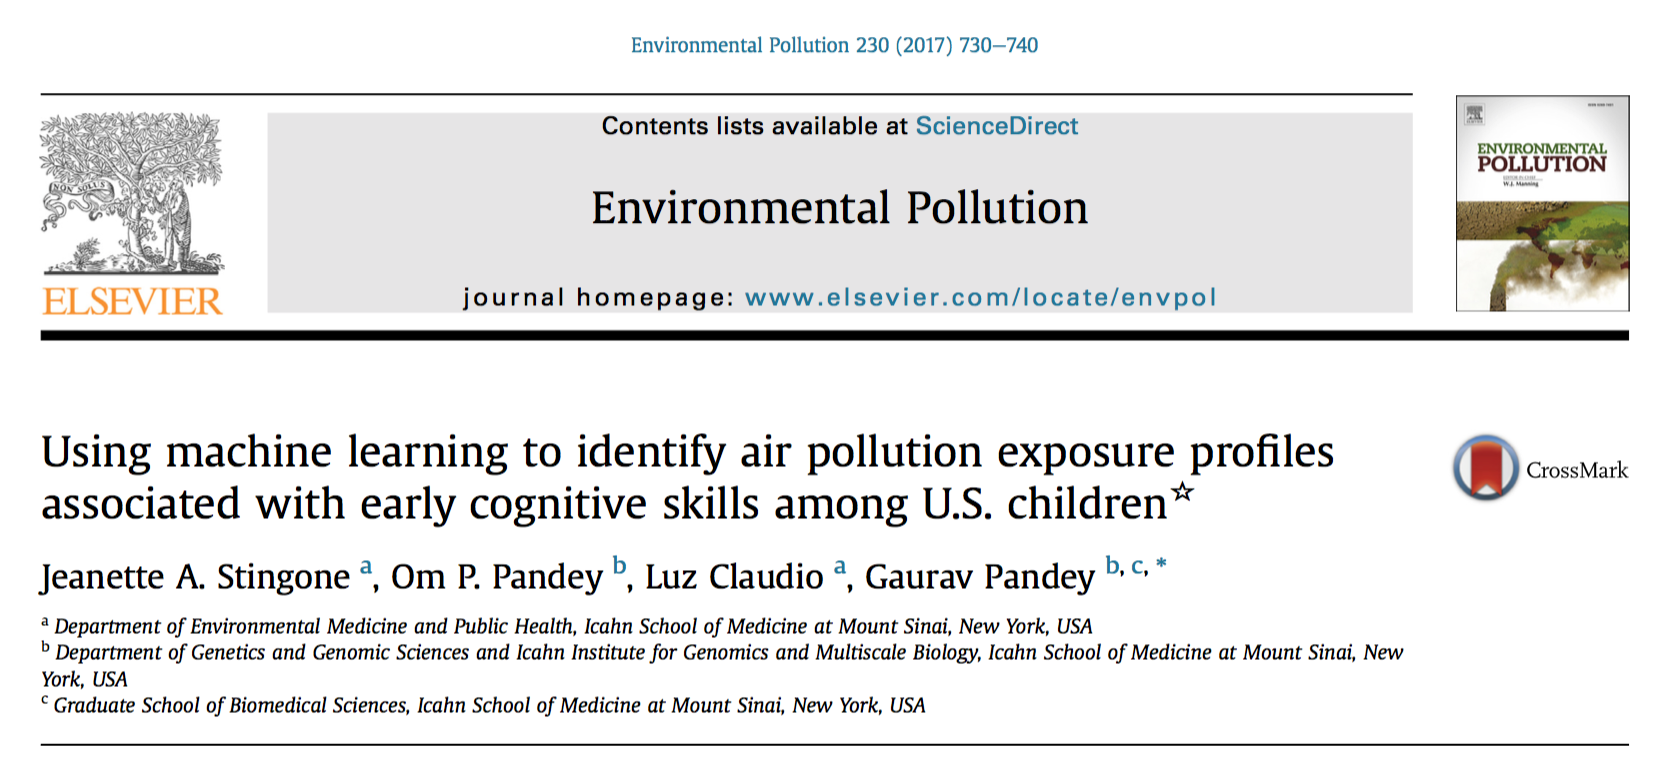
\includegraphics[width=\textwidth]{stingone_etal}
\end{frame}

\begin{frame}{Does pollution change cognitive ability?}

Stingone et al point out that few studies have looked at the effects of multiple pollutants at once

Key data:
\begin{itemize}
\item Kindergarten math scores from National Center of Education Statistics Early Childhood Longitudinal Study.  Randomly selected children.
\item Census tract estimates of 104 toxic pollutants from U.S. Environmental Protection Agency's National Air Toxics Assessment (NATA)
\item Other confounders including mother age, marital status, hhld income, etc.  (Used in second stage \textit{after} tree building.)
\end{itemize}

\end{frame}

\begin{frame}{Stingone \textit{et al} two step approach}

\begin{enumerate}
\item Build trees for test score outcome based on pollutant exposure (what we'll focus on here)
\item Run basic multiple linear regression \textit{within} each leaf to identify the effect of pollutants on test scores.  (We won't cover this part.)
\end{enumerate}
\end{frame}

\begin{frame}{Why trees?  Stingone \textit{et al's} justification}

\begin{itemize}
\item Easy interpretability in terms of understandable trees and/or rules, 
\item Ability to identify non-linear relationships between the features (exposures) and the outcome (math scores), 
\item Possibility of identifying interactions among the features (exposures), 
\item Making no/minimal assumptions about data distributions, 
\item Tolerance to missing values and outliers in the data, 
\end{itemize}
\end{frame}

\begin{frame}{Example result}

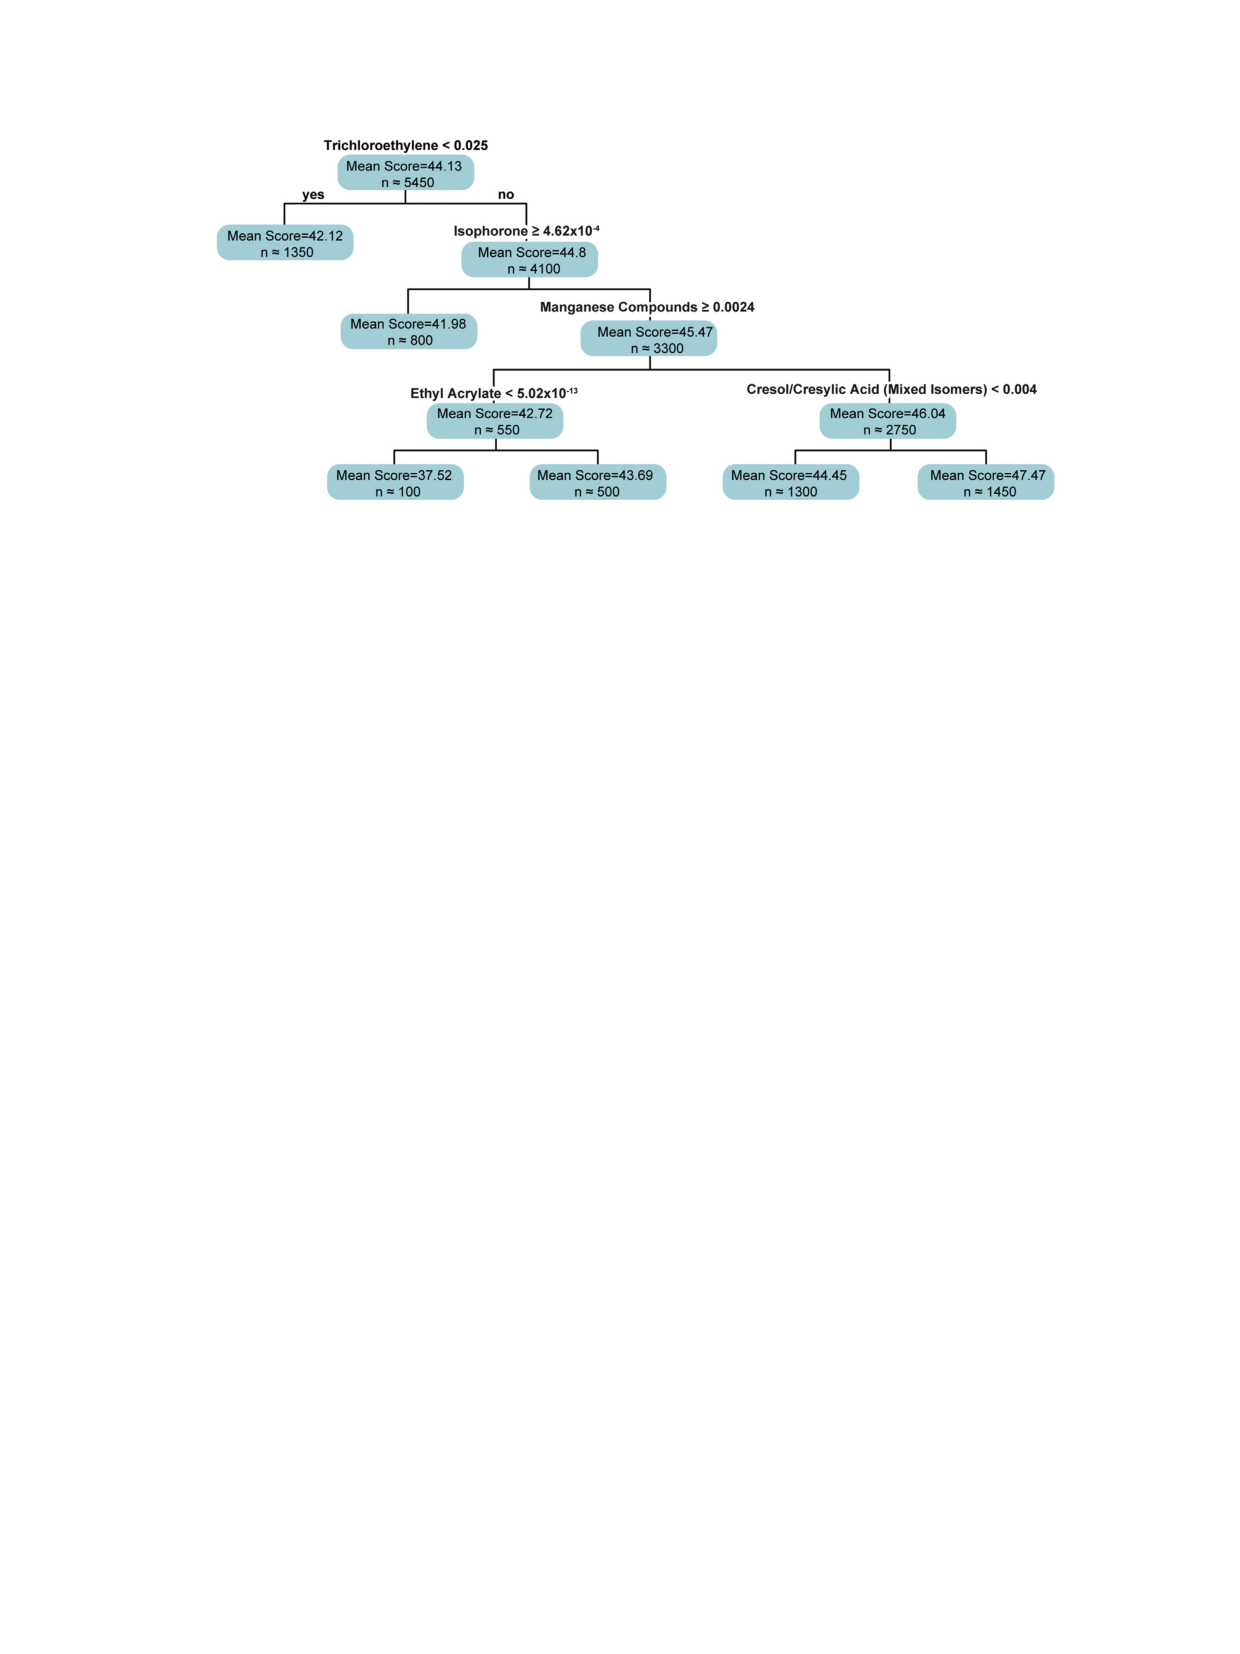
\includegraphics[width=\textwidth]{stingone_tree_totalpop}

Constructed with 10-fold cross-validation.  Also used additional random partitioning -- stay tuned.\\~\\

Note: $R^2$ values are low -- in this case 0.067.  Also note that in some cases \textit{lower} pollutant levels partition into \textit{lower} test scores.  Is this meaningful?
\end{frame}

\begin{frame}{A trick that Stingone \textit{et al }used}

They note that Trees are: 
\begin{itemize}
\item Prone to overfitting the (training) data, 
\item Sensitive to small perturbations in the data and/or model/algorithm parameters
\end{itemize}

Their approach to manage this is to build a lot of different trees using random partitions of the data.  \\~\\
Their approach is a little unconventional (for  reasons they don't provide).\\~\\

Instead, we'll soon talk about formal strategies to deal with this sensitivity -- boosting, bagging and random forests.  

\end{frame}

\begin{frame}
\begin{columns}
\column{0.5\textwidth}
\begin{center}
{\LARGE Classification trees} (Covered 11/8, not 11/6)
\end{center}
\column{0.5\textwidth}
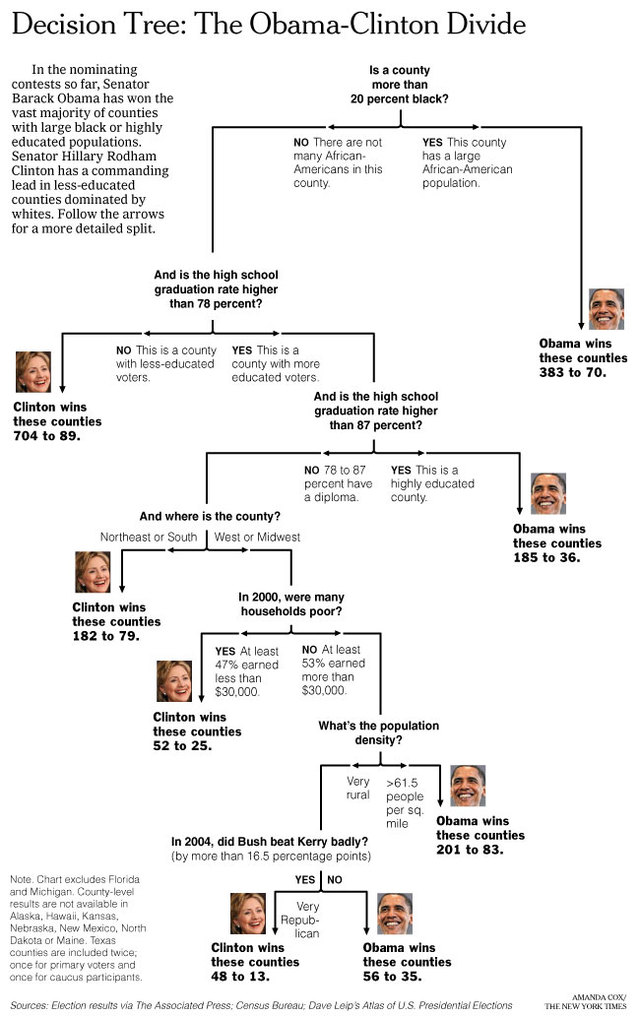
\includegraphics[height=\textheight]{NYT_tree}
\end{columns}
\end{frame}

\begin{frame}{What's a classification tree?}

As you might imagine, it's just like a regression tree, but we use it to predict a categorical or qualitative variable.  \\~\\

Rather than setting the prediction equal to the mean, the prediction is:
\pause
\begin{center}
 \textit{the most commonly occurring class within the partition.  \\~\\}
\end{center}

However we still use recursive binary splitting and cost-complexity pruning\\~\\

Though the \textit{criteria} for splitting and pruning will have to change

\end{frame}

\begin{frame}{What's the error?}

The typical error, $\text{RSS} = \sum_{i=1}^N (y_i-\hat{y}_i)^2$ won't work.  \\~\\

Alternatives?  Let's start by defining 
\begin{align*}
p_{mk} = \text{ fraction of observations belonging to class $k$ in region $m$.}
\end{align*}
Then a simple measure is:

\begin{center}
\textit{Classification error rate} = how many training observations don't fall into the assigned class.   \\~\\
\end{center}

 Within-region this is simply:

\begin{align*}
E_m = 1- \max_k (\hat{p}_{mk})
\end{align*}
\end{frame}

\begin{frame}{The trouble with Classification Error}

Suppose you have a two-class problem with 400 observations in each class.  Consider two possible splits (S1 and S2):
\begin{itemize}
\item[S1:] $R_1: (100,300)$, $R_2: (300,100)\Rightarrow \text{ weighted error } E_{S1} = 0.25$
\item[S2:]  $R_1: (200,400)$, $R_2: (200,0)\Rightarrow \text{ weighted error }E_{S2} = 0.25$\\~\\
\end{itemize}

Can you make a case for one of these being preferable to the other?\\~\\

\pause

S2 has a ``pure'' split, meaning there are \textit{no} errors in one of the splits.  You won't need to split this region any further.  

\end{frame}

\begin{frame}{Alternative errors}

Remember, $p_{mk} =$  fraction of observations in class $k$ in region $m$.

\begin{columns}
\column{0.5\textwidth}
\begin{figure}
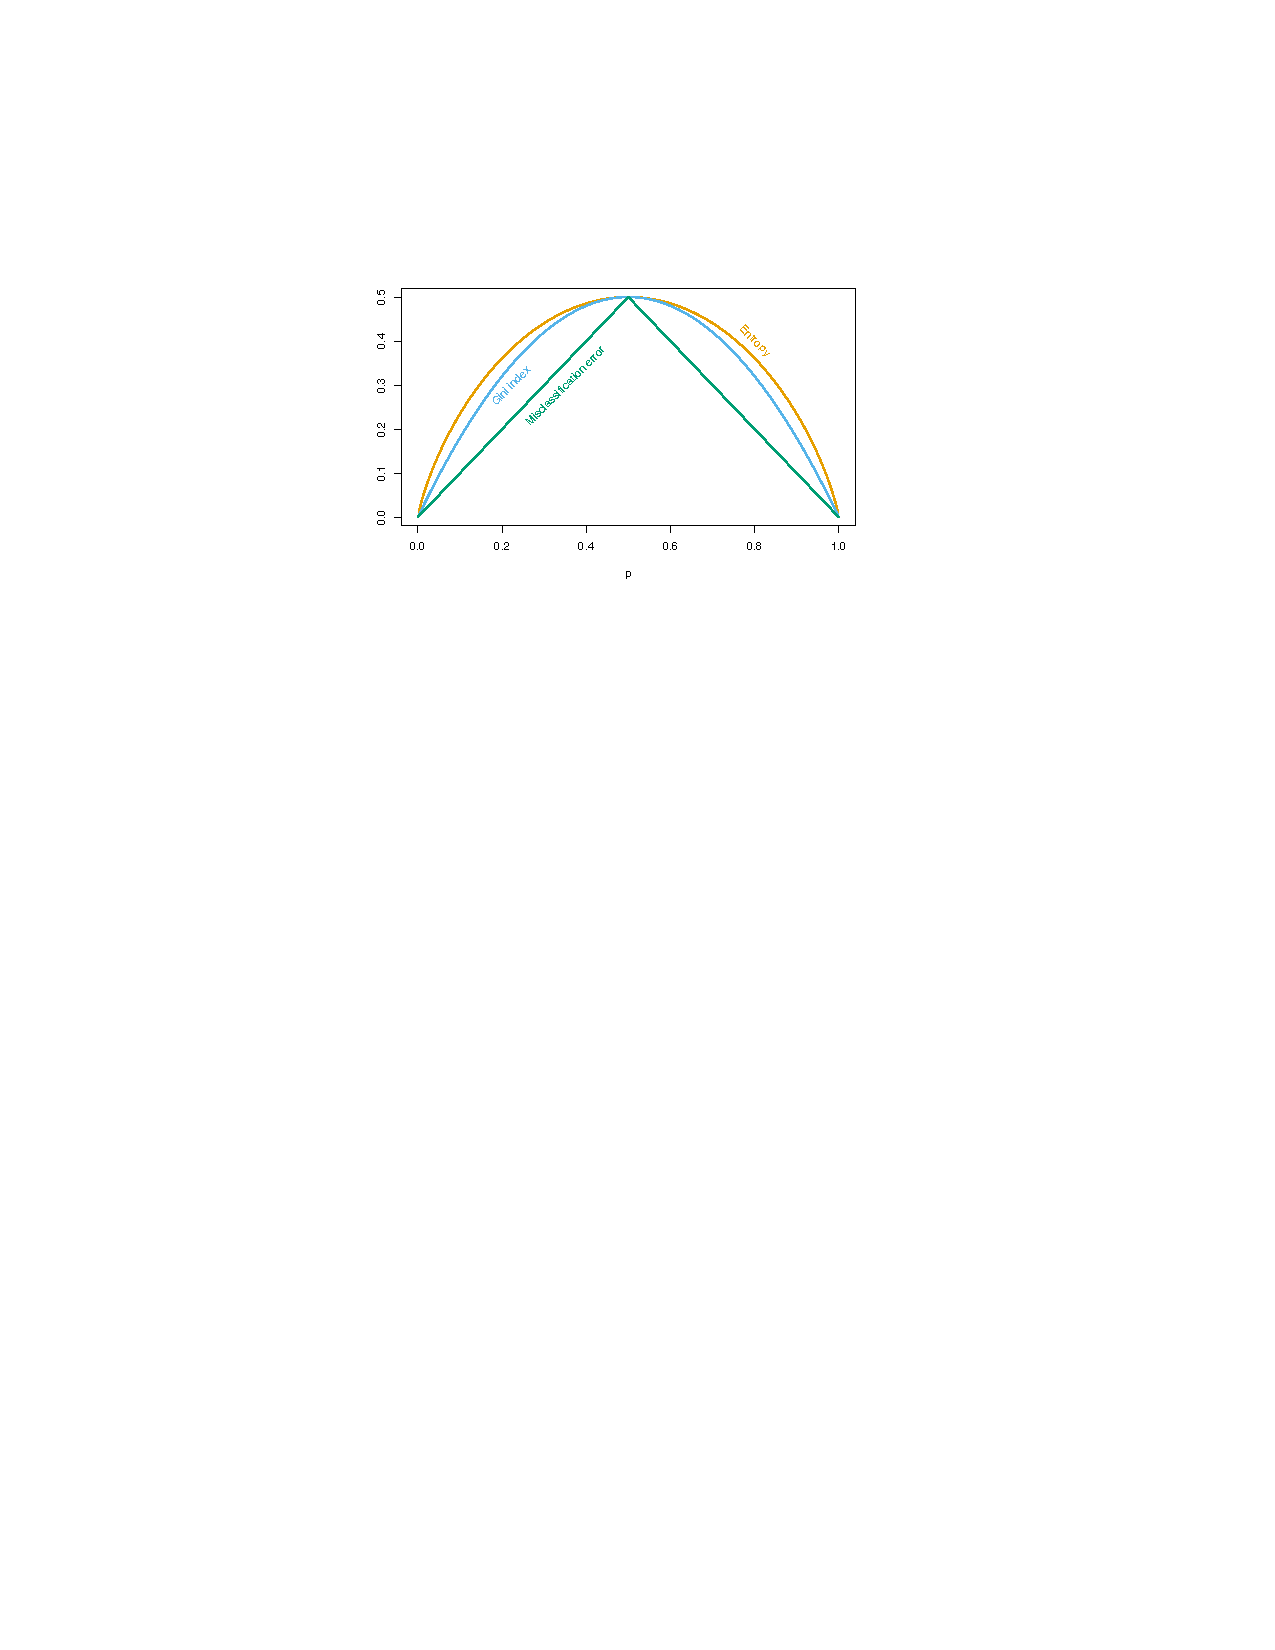
\includegraphics[width=0.9\textwidth]{E_vs_G_vs_D}
\vspace*{-3mm}
\caption*{\scriptsize (Measures for two-class classification; $p$ is the proportion in class 2. Cross-entropy scaled to pass through (0.5, 0.5).)}
\end{figure}
\column{0.5\textwidth}
\begin{align*}
E_m &= 1- \max_k (\hat{p}_{mk})\\
G_m &= \sum_{k=1}^K \hat{p}_{mk}(1-\hat{p}_{mk})\quad\text{``Gini''}\\
D_m &= -\sum_{k=1}^K \hat{p}_{mk}\log{ \hat{p}_{mk}}\quad\text{``Entropy''}
\end{align*}
\end{columns}
\vspace{-0mm}
$G$ and $D$ have two advantages:
\begin{enumerate}
\item Differentiable everywhere -- good for optimization
\item Score better for ``pure'' splits
\end{enumerate}
\end{frame}

\begin{frame}{Why do Gini and Entropy score pure splits better?}

\begin{columns}
\column{0.5\textwidth}
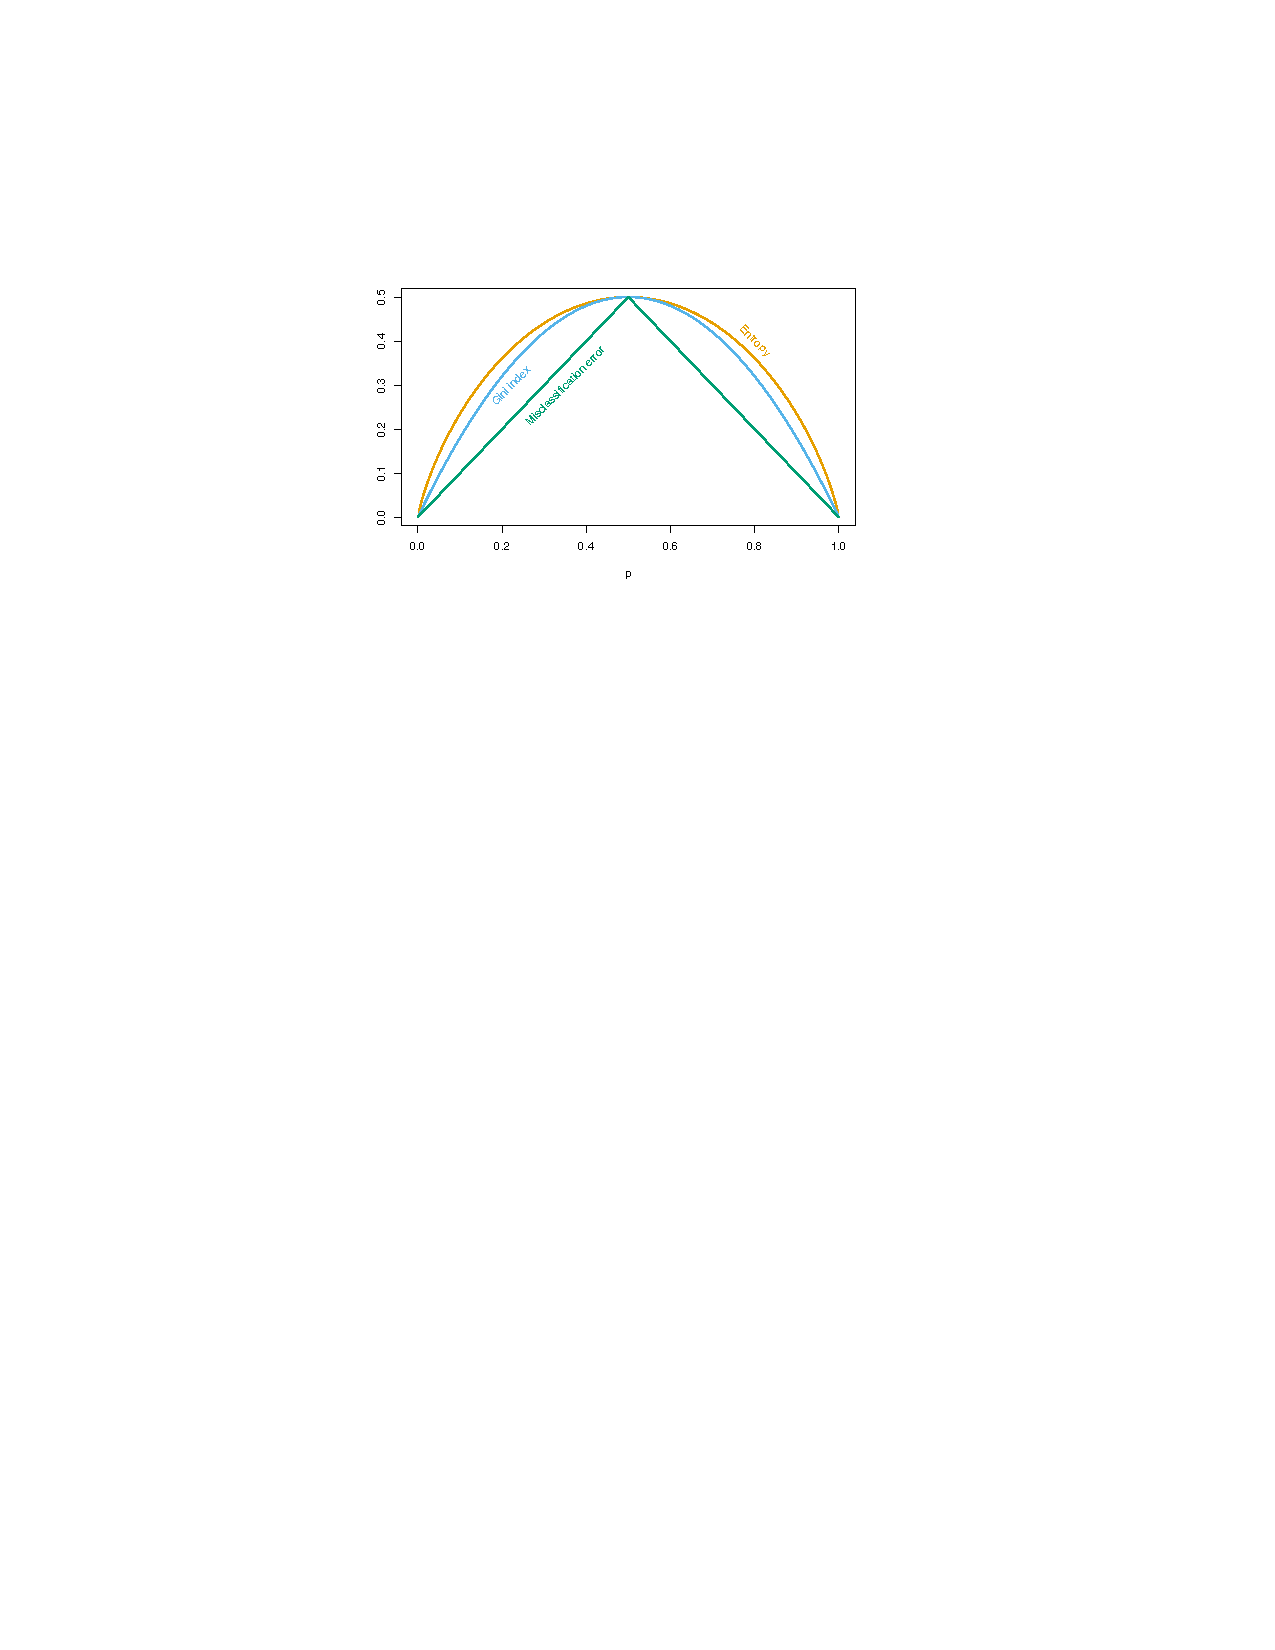
\includegraphics[width=0.9\textwidth]{E_vs_G_vs_D}

\column{0.5\textwidth}


\begin{itemize}
\item Misclassification indifferent between 
\begin{enumerate}
\item two regions with $p$ = 0.0 and $p$ = 0.4 or
\item two regions with $p$= 0.2 and $p$=0.2.
\end{enumerate}
\item ...but Gini and cross entropy would clearly prefer the first option.  
\end{itemize}
\end{columns}


\end{frame}

\begin{frame}{Which error rate to use?}

\begin{itemize}
\item Since they are more ``sensitive'' to pure splits, it's better to use either Gini or cross-entropy when \textit{growing} the tree. 
\item Any of the three measures can be used for cost-complexity pruning.  Common practice is to use the misclassification rate.
\begin{itemize}
\item That's because prediction is usually the final goal, and misclassification measures ability to do that.
\end{itemize}
\end{itemize}
\end{frame}


\begin{frame}{When are trees better than linear models?}
\begin{figure}
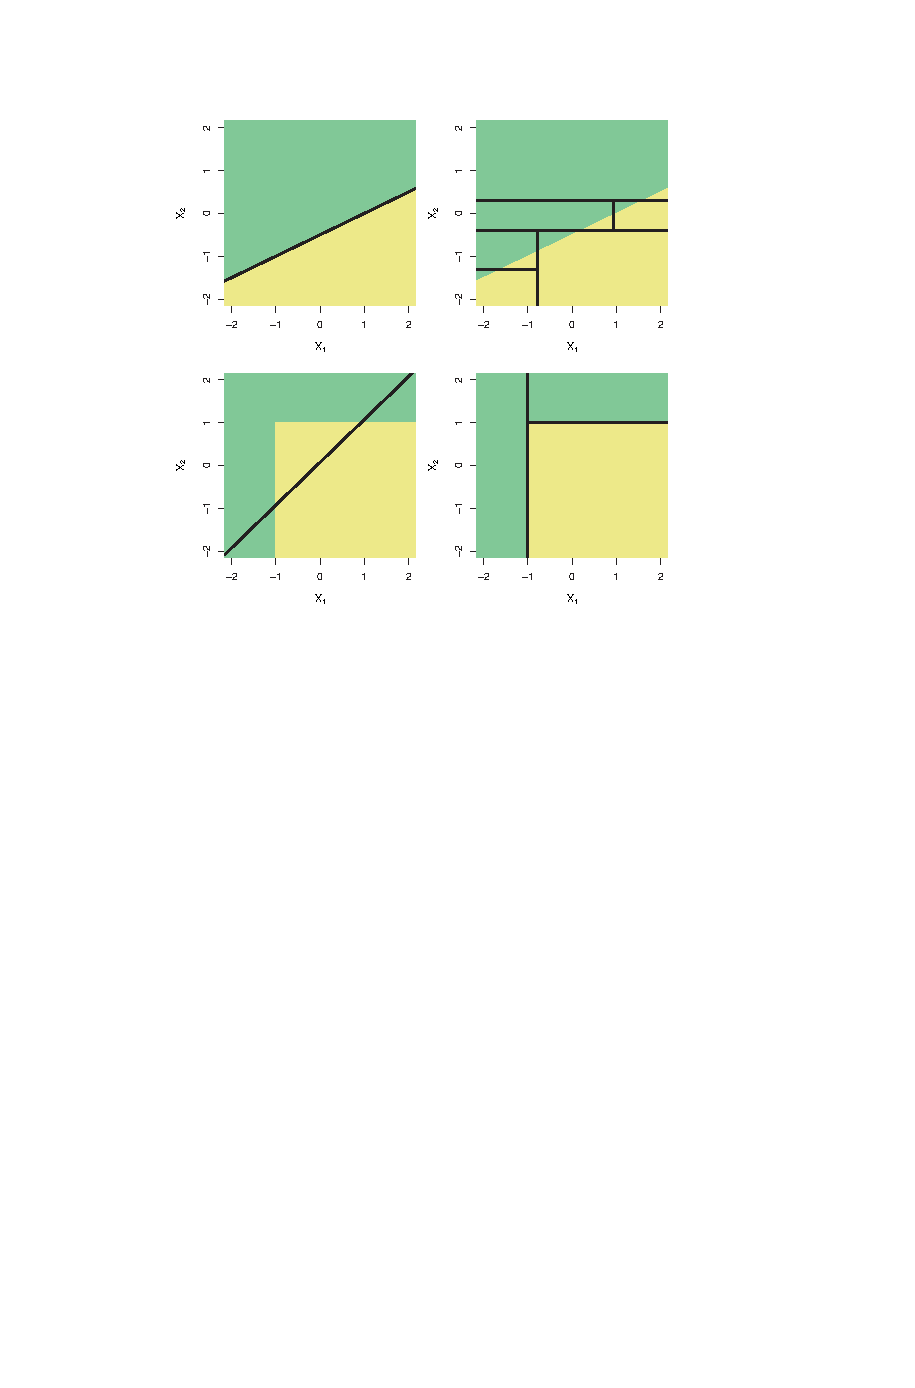
\includegraphics[height=0.9\textheight]{tree_vs_linear_for_classification}
\caption*{}
\end{figure}
\end{frame}

\begin{frame}{Reminder: advantages and disadvantages}
Advantages

\begin{itemize}
\item Easy to explain and non-experts can understand the results.
\item They're more like human decision-making.  Doctors like them.
\item They easily handle qualitative predictors -- no need for dummies.
\end{itemize}

Disadvantages

\begin{itemize}
\item As described, they don't usually provide the same predictive power that the other tools we've studied can.
\item They can be pretty sensitive to small changes in the data. 
\item Recursive binary splitting may generate a suboptimal tree (like forward / backward model selection).  Things later in the chapter address this.
\end{itemize}
\end{frame}

\begin{frame}{Supplemental Slides}

\end{frame}


\begin{frame}{A spam example}
Email data set, donated by George Forman from HP.  4601 messages.  

%\texttt{spam} = 1, \texttt{email} = 0

\begin{itemize}
\item 48 quantitative predictors: the percentage of words in the email that match a given word. Examples include business, address, internet, free, and george. (These could be customized for individual users.)
\item 6 quantitative predictors: the percentage of characters in the email that match a given character. The characters are ch;, ch(, ch[, ch!, ch\$, and ch\#.
\item The average length of uninterrupted sequences of capital letters: CAPAVE.
\item The length of the longest uninterrupted sequence of capital letters: CAPMAX.
\item The sum of the length of uninterrupted sequences of capital letters: CAPTOT.
\end{itemize}

\end{frame}

\begin{frame}{}
\begin{figure}
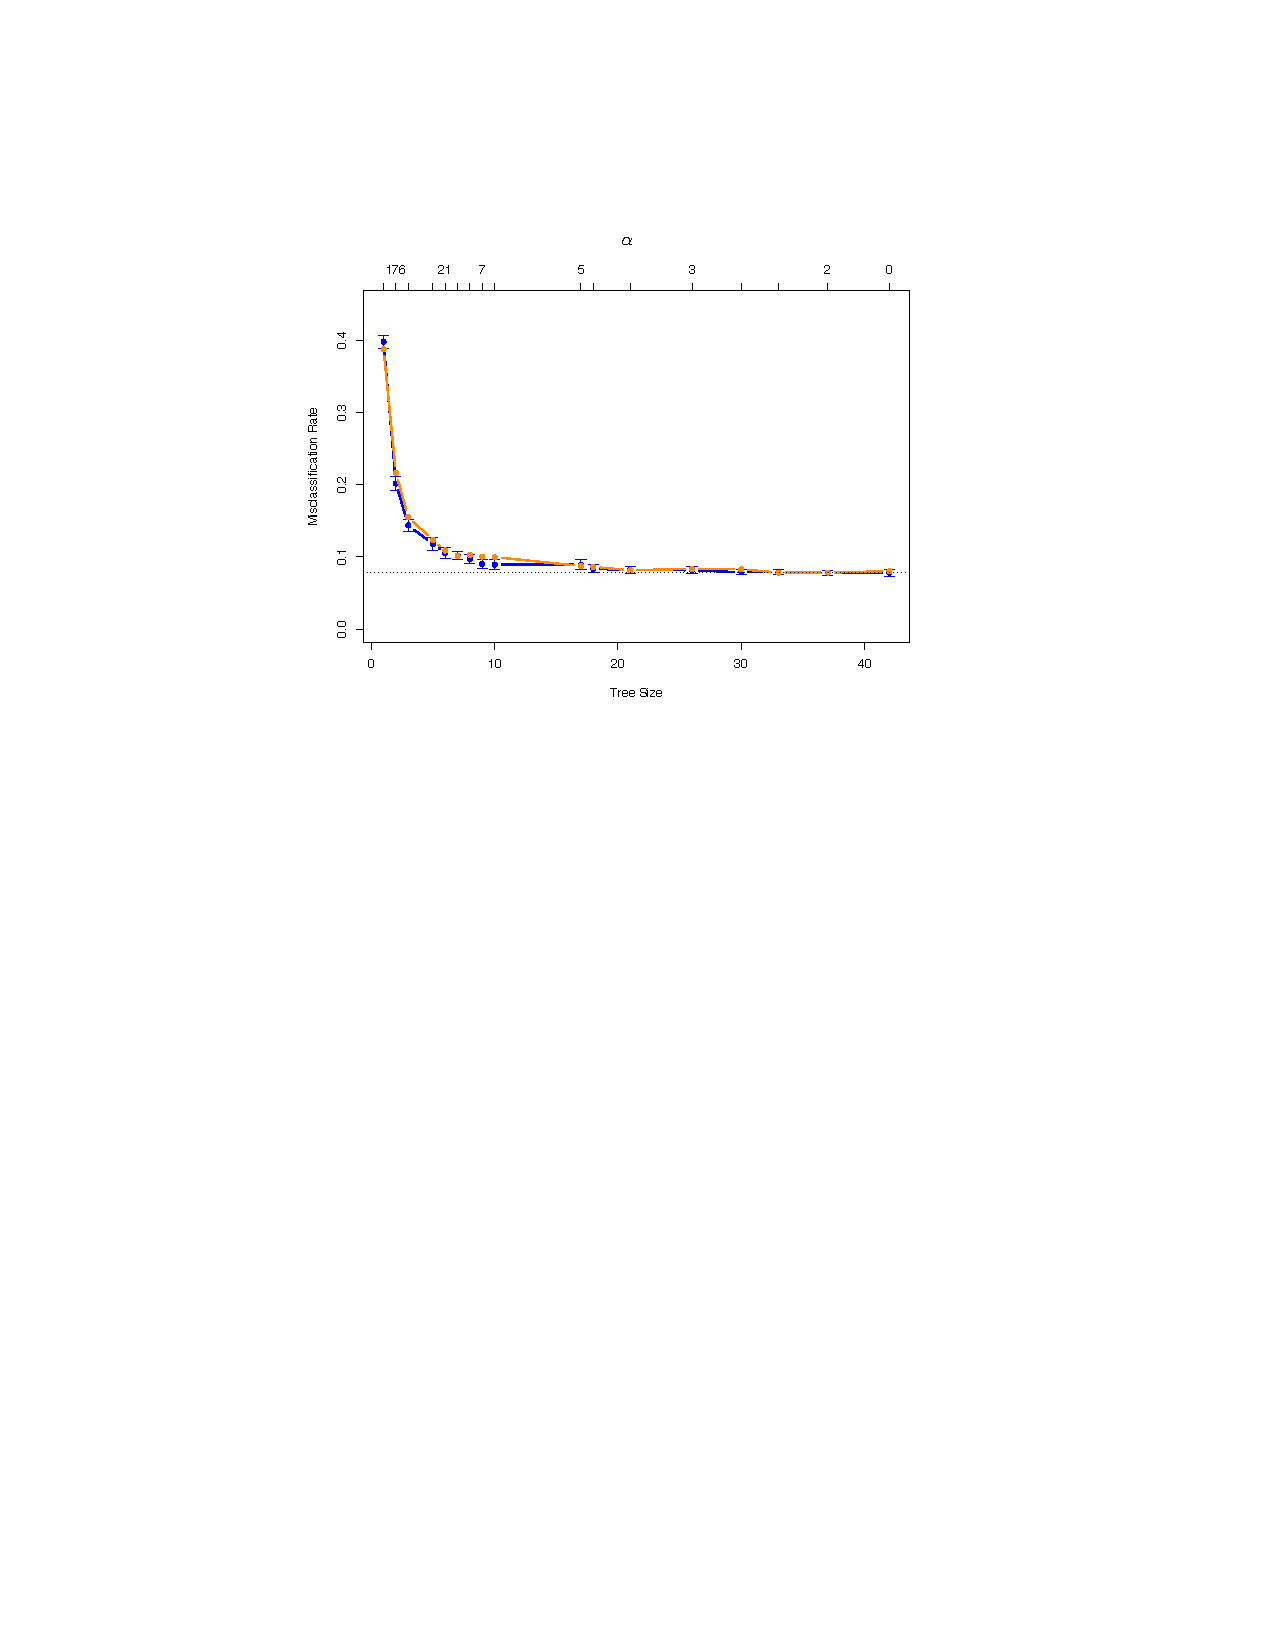
\includegraphics[width=0.8\textwidth]{spam_error}
\caption*{Blue: test data set error indexed by tree size.  Orange: 10-fold CV error indexed by $\alpha$.  Minimum (within 1 standard error) is at $|T|=17$.  Figure from ESLII}
\end{figure}
\end{frame}

\begin{frame}{}
\begin{figure}
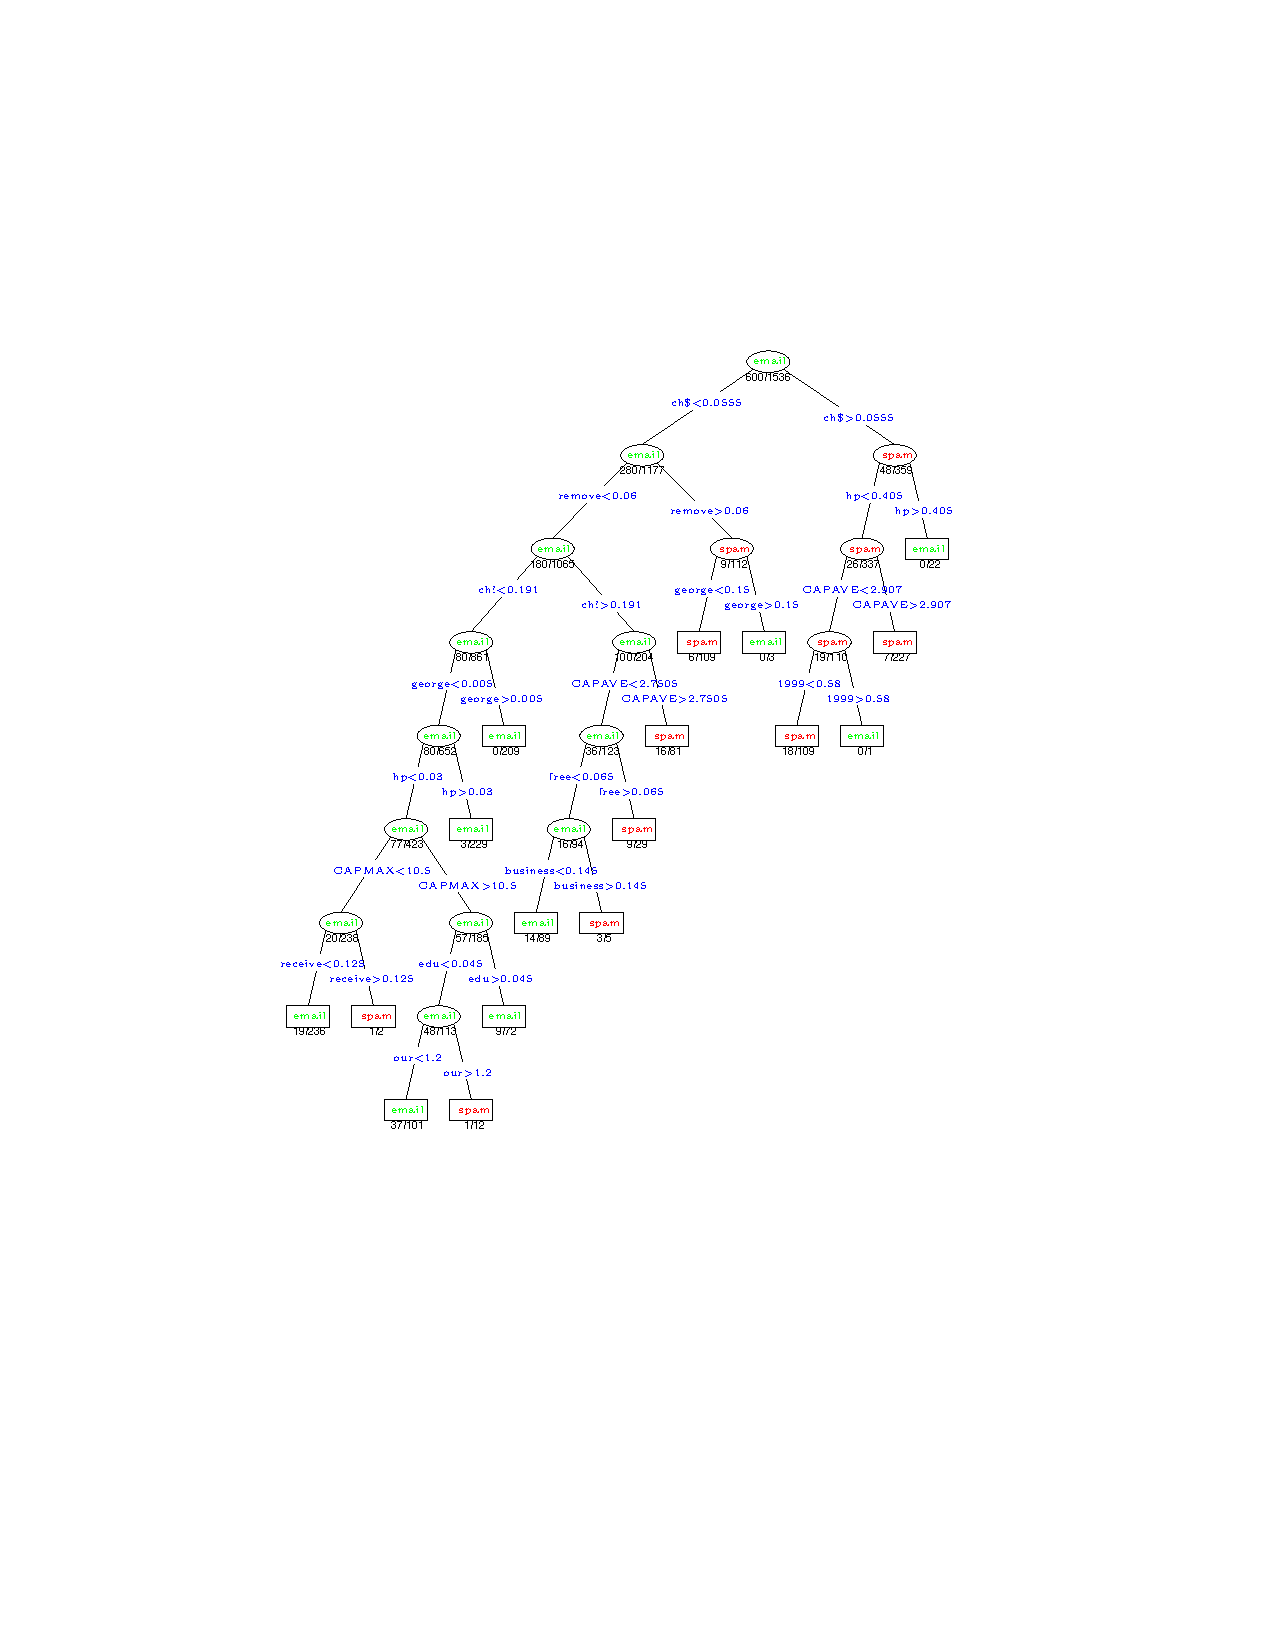
\includegraphics[height=0.93\textheight]{spam_tree}
\caption*{ Figure from ESLII}
\end{figure}


\begin{textblock*}{50mm}(75mm,55mm)
\begin{exampleblock}{}
\scriptsize
\begin{itemize}
\item Split variables are shown in blue on the branches, 

\item Classification is shown in every node in red or green.

\item The numbers under the terminal nodes indicate misclassification rates on the test data.
\end{itemize}

\end{exampleblock}
\end{textblock*}

\end{frame}

\begin{frame}{A zoom in}

\vspace*{-10mm}
\begin{figure}
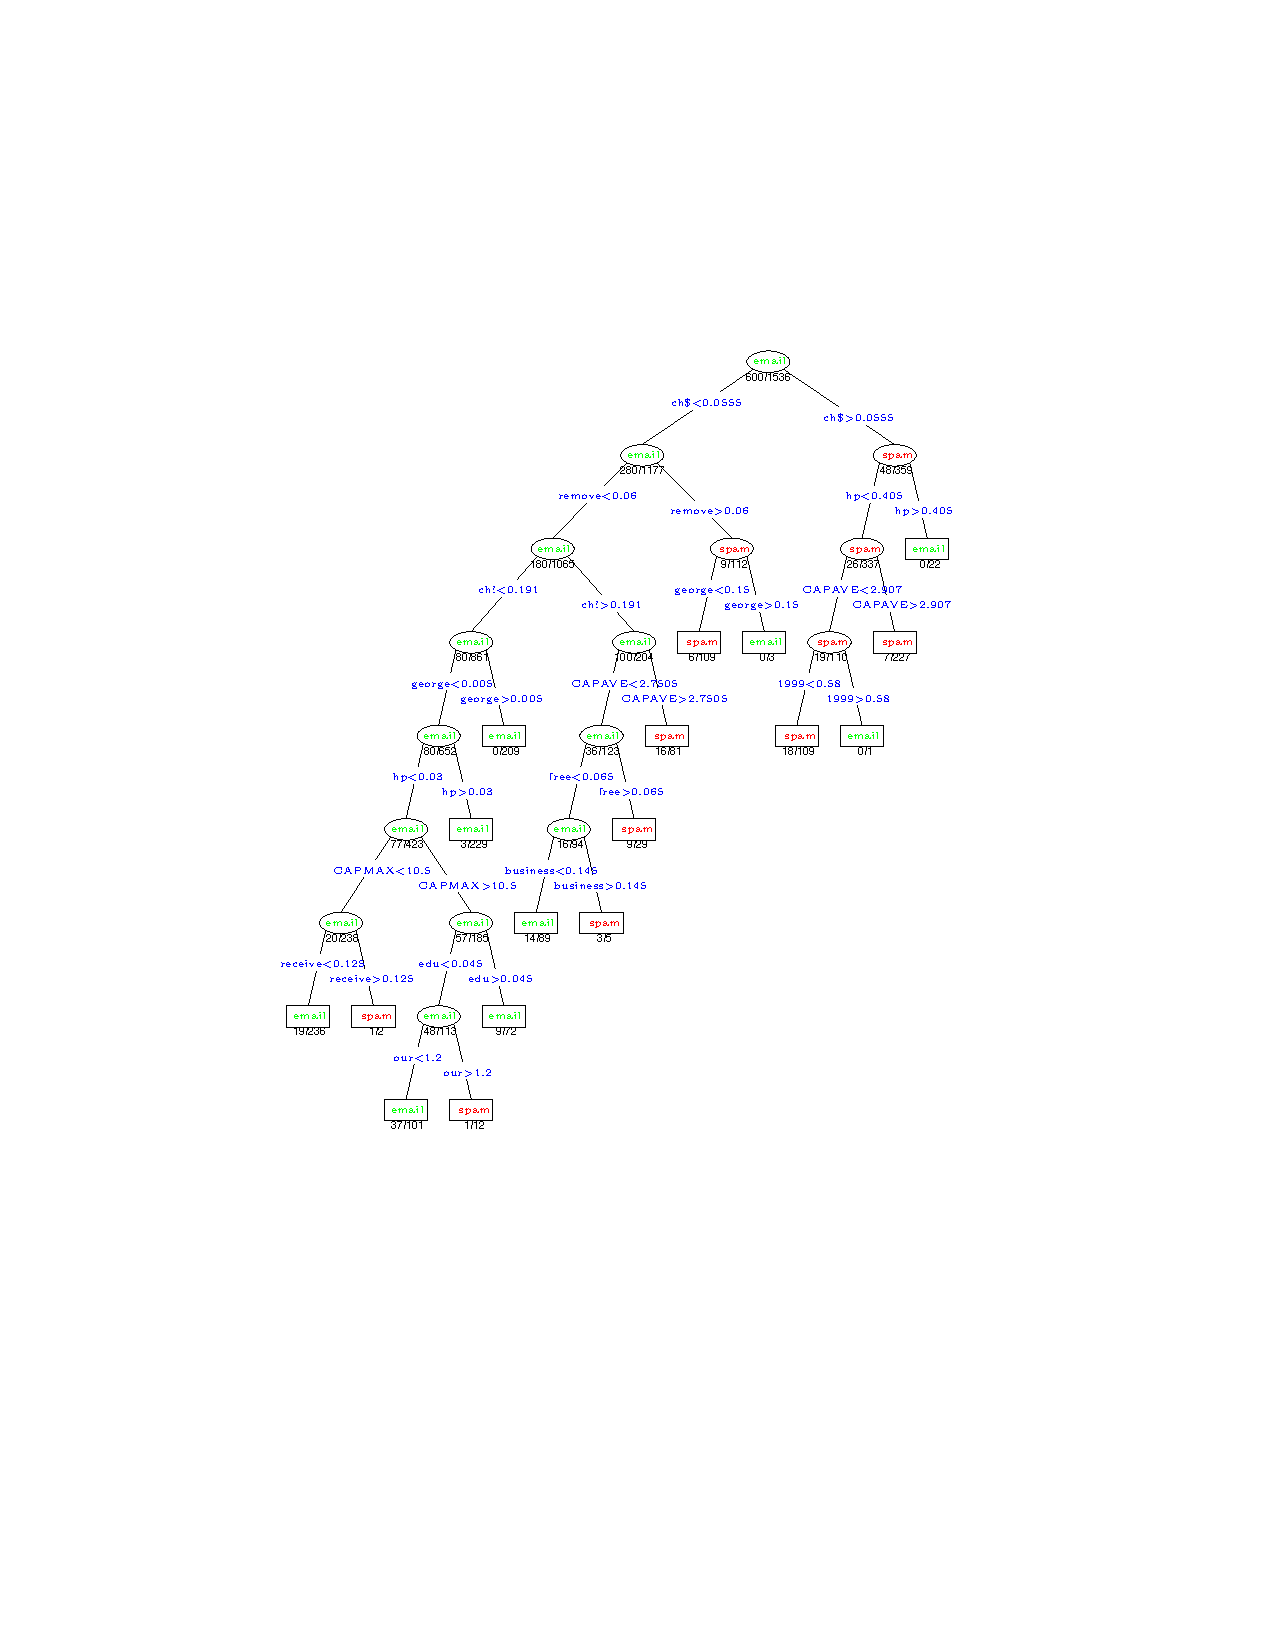
\includegraphics[height=1.5\textheight]{spam_tree}
\caption*{ Figure from ESLII}
\end{figure}
\end{frame}
\end{document}
